\cotefile{136}
\scanpage{343}
% The first group is enclosed by a single freehand line.
\noindent\fbox{\begin{minipage}{.94\linewidth}
\diagram{\begin{tikzcd}[ampersand replacement=\&,column sep=small,row sep=small]
 A \arrow[r,"u_i"] \arrow[d] \& B \arrow[d] \& \deleted{\unsure{\sum}}\quad k[T] \arrow[r,"u_i",dash] \& B\\
 K \arrow[r,hook,-] \& K' \& T \arrow[r,|-] \& b_i\\
 {} \& \& T^n \arrow[r,dash] \& b_i^n
\end{tikzcd}}
\hfill\unsure{intègre|\(i\) distincts|injectif}\hfill\mbox{}
\[
 Y\longleftarrow X_{\unsure{*|+}}\qquad\qquad \sum\lambda_i b_i^n=0
\]
\[
\begin{aligned}
 \sum\lambda_i u_i&=0 & \operatorname{Ker}u_i&=\mathfrak p_i\quad\text{idéal premier}\\
 &&\deleted{\unsure{\text{soit}}}\ t&\in\unsure{\complement}\bigcup\mathfrak p_i
       =\bigcap\unsure{\complement}\mathfrak p_i\\
 \sum\lambda_i u_i(x)^n&=0 & &\forall n
\end{aligned}
\]
\[
 \deleted{u_i=u_j}\quad u_i(x)-u_j(y)
\]
\end{minipage}}

\[
 \operatorname{Hom}(\Delta^{m}_{\unsure{*}},\Delta^{n}_{\unsure{*}})
 \xrightarrow{\sim}\operatorname{Hom}_{\mathrm{mult}}
 (F_{(\Delta^n_{*})},F_{(\Delta^m_{\unsure{*}})}).
\]

\[
 X_*\longrightarrow\widetilde X_*=n\longmapsto
 \operatorname{Hom}(F_{X_*},F_{\Delta^n_*})
\]
\margin{\(\shortparallel\)\quad\deleted{\(n\mapsto X_n\)}}
\diagram{\begin{tikzcd}[ampersand replacement=\&,row sep=small]
 {}\\
 \operatorname{Hom}\bigl(\varprojlim_{\Delta^m_*/X_*} F_{\Delta^m_*},F_{\Delta^n}\bigr)
 \arrow[u,phantom,"\rotatebox{90}{=}" description]\\
 \varinjlim_{\Delta^m_*/X_*}
 \underbrace{\operatorname{Hom}(F_{\Delta^m_*},F_{\Delta^n})}
 \arrow[u,"\text{\textcircled{\scriptsize Iso?}}"']\\
 {\operatorname{Hom}(\Delta^n_*,\unsure{{}'\Delta^m_*|\Delta^m_*})
 =\Delta^m_{[n]}}\arrow[u,phantom,"\rotatebox{90}{=}" description]\\
 X_{[n]}\arrow[u,phantom,"\rotatebox{90}{=}" description]
\end{tikzcd}}

Soient \deleted{\unsure{deux|donc}}
\diagram{\begin{tikzcd}[ampersand replacement=\&,column sep=large]
 \overset{\unsure{G}}{\overset{\shortparallel}{\prod F_i}} \arrow[r] \arrow[d,"\mathrm{pr}_i"'] \& F_{\Delta n}
 \& \prod G_i^{\bullet}\arrow[r,dash] \& C^{\bullet}_{[n]}\\
 F_i \arrow[ur,"u_i"] \& \deleted{\sum\lambda_i u_i} \& \forall M_* \&
\end{tikzcd}}
\[
 \deleted{\unsure{\mathrm{Gr}}\,\unsure{F_i}(M_*)\longrightarrow F(M_*)}
\]
\[
 \operatorname{Sym}\unsure{G_i|G}(M_*)\xrightarrow{u_i}\deleted{\operatorname{Sym}}F(M_*)
\]
% archive sheet number: 344
\scanpage{345}
\deleted{\(F(X_*)= \)} \(C^\bullet(X_*)\) avec sa structure mult et à puiss. div
\[
\begin{aligned}
 F_*(X_*)&=[n\longmapsto\operatorname{Hom}(C^\bullet(X_{\unsure{*|\bullet}}),C(\Delta^n_*))\\
 F_*(\Delta^{m}_{{\deleted{\unsure{[n]}}}*}\deleted{{}^{*}})
 &=P^m_{\deleted{\unsure{[n]}}*}=\rho_*^{m\,-1}(T)
\end{aligned}
\]
torseur sous \(\check\Psi_m\otimes\Phi_*=\Phi_*^{m+1}\)
(dont le groupe des sections est \(k^{m+1}=\check\Psi_m\))
\[
\begin{aligned}
 \rho^m_*\colon\quad\check{\Phi}_m\otimes\Phi_*&\longrightarrow\Phi_*.
 \quad\text{(\unsure{s'insérant dans})}\\
 0\;-\;\check\Psi_m\otimes\Phi_* \;-\;
 \underbrace{\check{\Phi}_m\otimes\Phi_*}_{
 \operatorname{Hom}(\Phi_m,\Phi_*)\,;\ T_m\mapsto T_*}
 &\;-\;\Phi_*\;-\;0
\end{aligned}
\]
\diagram{\begin{tikzcd}[ampersand replacement=\&,column sep=small]
 \Delta^m_{\deleted{\unsure{n}}*}\arrow[r,"y"] \& P^m_* \& y\in P^m_m\\
 \deleted{\Delta^m_n=\operatorname{Hom}_{\mathrm{ens}}(\Delta^n,\Delta^m)}
 \arrow[r,"\deleted{\unsure{y}}"] \arrow[dr,bend right] \& P^m_n \&\\
 {} \& {\operatorname{Hom}(P^m_*,P^n_*)}\arrow[dr,bend right] \&\\
 {} \& {} \& \unsure{\operatorname{Hom}(P^m)|\operatorname{Hom}(P^n)}
\end{tikzcd}}
\[
 \begin{aligned}
 F_*(X_*)&=\operatorname{Hom}\bigl(\varprojlim_{\unsure{\Delta^m_*\in\mathrm{Ob}\,\Delta_{/X_*}}}
 \deleted{\unsure{\lim}} C^\bullet(\Delta^m_*),C^\bullet(\Delta^*_* )\bigr)\\
 &\hspace{1em}\uparrow\quad\text{\unsure{isom ou|une va|est-ce une} équiv. d'homotopie ?}\\
 &\varinjlim_{\Delta^m_*\in\mathrm{Ob}\,\Delta_{/X_*}}\operatorname{Hom}
 \bigl(\deleted{\unsure{\lim}}(C^\bullet(\Delta^m_*),C^\bullet(\Delta^*_*))=
 \varinjlim_{\Delta^m_*\in\mathrm{Ob}\,\Delta_{/X_*}}P^m_*\\
 &\hspace{1em}\uparrow\\
 &\varinjlim_{\Delta^m_*\in\mathrm{Ob}\,\Delta}\Delta^m_*
 \end{aligned}
\]
\[
 \begin{array}{ccc}\Phi_m&\longrightarrow&\Phi_m\\ T_m&&T_m\end{array}
 \qquad \alpha\in k,\quad\beta\in\overline{T}_m
\]
\[
 \begin{array}{ccc}
 T_i&T_i\circ T_1&\cdot\\ y&T_i\circ y&y\circ T_1\\ &y\circ y&
 \end{array}
\]
\[
 \begin{aligned}
 X_*&=\operatorname{Coker}\bigl(\Delta^0_*\overset{\partial_0,\partial_1}{\rightrightarrows}\Delta^1_*\bigr)\\
 C^\bullet(X_*)&=\operatorname{Ker}\bigl(C^\bullet(\Delta^1_*)
 \overset{C^\bullet(\partial_0),C^\bullet(\partial_1)}{\rightrightarrows} C^\bullet(\Delta^0_*)\bigr)
 \end{aligned}
\]
\diagram{\begin{tikzcd}[ampersand replacement=\&,column sep=small,row sep=small]
 0\arrow[d] \& 0\arrow[d] \& 0\arrow[d] \& 0\arrow[d]\\
 \Phi_m \arrow[d] \&
 k \arrow[l,"{\alpha T_m\mathrel{\longleftarrow\!\shortmid} 1=T_i}"'] \arrow[d,"0"']\arrow[r,"\mathrm{diag}"] \&
 \Phi_1=k^2 \arrow[d,"\unsure{\wedge T_1}"] \arrow[r,bend left,"{\partial_0^*=\mathrm{pr}_0}"]
 \arrow[r,bend right,"{\partial_1^*=\mathrm{pr}_{\unsure{1|*}}}"'] \&
 \Phi_0=k \arrow[d]\\
 \bigwedge^2\Phi_m\arrow[d] \& k\arrow[l,"{T_m\wedge\beta\mathrel{\longleftarrow\!\shortmid} 1}"']\arrow[d]\arrow[r,"\mathrm{id}","\sim"'] \&
 \bigwedge^2\Phi_1=k\arrow[d] \& 0\\
 0 \& 0 \& 0 \&\\
 {(\beta\in\Phi_m)} \& {} \& {} \&
 \end{tikzcd}}
\[
 k\qquad F_*(X_*)=\operatorname{Hom}\bigl(
 [0-k\xrightarrow{0}k\longrightarrow 0\longrightarrow\cdots0],
 C^\bullet(\Delta^*_*))=
 \bigl\{n\longmapsto\operatorname{Hom}([\;-\;],
 [\Phi_n\longrightarrow\bigwedge^2\Phi_n\longrightarrow\cdots)\bigr\}
\]
(structure mult. induite par \(C^\bullet(\Delta^1_*)\))
\[
 \alpha\in k\qquad \beta\in T
\]
% archive sheet number: 346
\scanpage{346}
\[
 d,\ \lambda=\overline T_{\wedge},\ \delta,\ \mu_j=T_{\cdot}^{\unsure{(i)|(j)}},\quad
 \Theta(x)=\deg(x)\,x
\]
\[
 1,T,\overline T,\qquad
 \deleted{\bigwedge^{\unsure{i}}\varphi\otimes\bigwedge^{\unsure{j-1}}\psi}
 \qquad\unsure{\bigwedge}
\]
\[
\left\{\begin{aligned}
 d\lambda+\lambda d&=0 &&*\\
 d\delta+\delta d&=\Theta\quad\text{en degré total}.\\
 \delta\lambda+\lambda\delta&=\mu\\
 d\mu_i-\deleted{\unsure{\lambda\mu_i+}}\mu d&=\unsure{\mu_{i-1}|\lambda\mu_{i-1}}\lambda\\
 \lambda\mu_i-\mu_i\lambda&=0 &&*\\
 \delta\mu_i-\mu_i\delta&=0 &&*
\end{aligned}\right.
\qquad
\left\{\begin{aligned}
 d\Theta-\Theta d&=0 &&*\\
 \delta\Theta-\Theta\delta&=0 &&*\\
 \Theta\lambda-\lambda\Theta&=\lambda\\
 \unsure{\Theta_i|\Theta}\mu_i-\mu_i\Theta&=i\mu_i
\end{aligned}\right.
\]
\[
\begin{aligned}
 d(T^{(i)}x)&=\underbrace{d(T^{(i)})}_{\unsure{\lambda T^{(i-1)}\overline T_{\wedge}}}x+T^{(i)}dx
 \qquad d^\alpha\delta^\beta\lambda\\
 d\mu_i(x)&\\
 \delta(Tx)&=\deleted{\delta(T)x}+T\delta x
\end{aligned}
\]
\[
 \boxed{\begin{aligned}
 \Theta\mu_f-\mu_f\Theta&=\mu_{\Theta f}\\
 d\mu_f-\mu_f d&=\mu_{f'}\lambda
 \end{aligned}}
\]
\[
 \underline{d\quad\lambda}\qquad\underline{\lambda\quad\mu},\quad
 \underline{\mu\ \delta}
 \qquad \frac{n(n-1)}2=\frac{5\cdot4}2=10
\]
\[
 \underbrace{\underbrace{d\lambda}\underbrace{\mu\delta}}_{0}
 \qquad \frac{n(n-1)}2=\unsure{45}
\]
\[
 d\ \delta\ \lambda\ \overset{i\geq1}{\mu_i}\ \Theta\qquad d,\delta,\lambda
\]
\[
 \left\{\begin{aligned}
 d^2&=\delta^2=\lambda^2=0\\
 \mu_i\mu_j&=\unsure{C_{ij}|C^i_{i+j}}\mu_{i+j}
 \end{aligned}\right.\qquad
 \Theta^2\quad\text{\unsure{rien au dessus}}
\]
\[
 \begin{aligned}
 \unsure{\varphi|\Theta}(\lambda x)&=(\deg x+i)\lambda x\\
 \lambda(\varphi x)&=\deg x\ \lambda x\\
 \varphi\lambda-\lambda\varphi&=i\lambda x
 \end{aligned}
\]
\[
 \underbrace{\overbrace d^{\cdot}\ \overbrace\lambda^{\cdot}\
             \overbrace{\mu_f}^{\cdot}\ \overline\delta}_{\Theta}
 \quad \delta(T^{(i)})=0\qquad
 \left\{\begin{aligned}
 d^2&=\delta^2=\lambda^2=0\\
 \mu_{f}\mu_{g}&=\mu_{fg}\qquad \mu_f,\ \unsure{f\in\Gamma}\\
 \Theta^2&=\text{---}
 \end{aligned}\right.
\]
\[
 \sum^{\unsure{de}}\lambda^\epsilon\cdot\mu_{f(\epsilon)}\ ;\ \delta^{\epsilon'}\Theta.
 \quad
 \left\{\begin{aligned}
 \boxed{d\delta+\delta d=\Theta}&\\
 \delta\lambda+\lambda\delta&=\mu_T && \delta(\overline T)=\unsure{T|1}\\
 d\mu_f-\mu_f d&=\mu_{f'}\lambda\\
 \Theta\lambda-\lambda\Theta&=\lambda\\
 \Theta\mu_f-\mu_f\Theta&=\mu_{\Theta f}
 \end{aligned}\right.
\]
\[
 \sum_{\substack{\deleted{\unsure{\alpha,\beta,\sigma,n}}\\
  \alpha,\beta,\sigma\in\mathbb F_2\\n\in\mathbb N}}
 \mu_{f_{\alpha,\beta,\sigma,n}}\underbrace{\lambda^\alpha d^\beta\delta^\sigma\Theta^n}_{
 \unsure{f_{\epsilon,\epsilon',\epsilon'',n}}\lambda^\epsilon d^{\epsilon'}\delta^{\epsilon''}\Theta^n}
 \qquad\deleted{\unsure{\mu_g}}
\]
\[
 \begin{aligned}
 f\,\lambda^\alpha d^\beta\delta^\sigma\Theta^n\,g\,
 \lambda^{\alpha'}d^{\beta'}\delta^{\sigma'}\Theta^{n'}\\
 \lambda^\alpha
 \underbrace{d^\beta g}_{g d^\beta+\beta g'\lambda}
 \delta^\sigma\lambda^{\alpha'}d^{\beta'}\delta^{\sigma'}
 \end{aligned}
\]

Cas \(p\) quelconque \(\inserted{\geq1}\), \(q=1\)
\diagram{\begin{tikzcd}[ampersand replacement=\&,column sep=small]
 0\arrow[r,dash] \&\Gamma^p\Phi_*\arrow[r] \&
 \Gamma^p\Phi_*\otimes\Phi_*\arrow[r,dash] \&
 \Gamma^p\Phi_*\otimes\Psi_\alpha\arrow[r]\arrow[l,bend left,"?"'] \&0\\
 {} \& {} \& {} \& \Phi_\alpha\times\Psi_\alpha' \arrow[ul] \&
\end{tikzcd}}
\[
 (\varphi,\psi)\longrightarrow s(\varphi\otimes\psi)\varphi^{(p-1)}
\]
\diagram{\begin{tikzcd}[ampersand replacement=\&]
 \Gamma^{\deleted{\unsure{*}}\,\cdot+}\Phi_*\otimes
 \bigwedge^{*}_{\deleted{\unsure{*}}}\Psi_\alpha \arrow[d]\\
 \Gamma^{*+}\Phi_\alpha\otimes\bigwedge^{<}\Phi_\alpha
\end{tikzcd}}
\[
 \varphi_1^{\deleted{\unsure{2}}(p_1)}-\varphi_r^{(p_r)}
 \qquad \sum p_i=p\qquad \Big\downarrow
\]
\[
 \begin{aligned}
 &\sum\lambda_i\varphi_i\,-\\
 f\left(\sum_1^r\lambda_i\varphi_i\right)
 &=s\left(\sum\lambda_i\varphi_i\otimes\psi\right)
       \left(\sum\lambda_i\varphi_i\right)^{(p-1)}\\
 &=\sum_{1\leq i\leq r}\lambda_i s(\varphi_i\otimes\psi)
 \sum_{\substack{(p_1,\ldots,p_r)\\\in\mathbb N^r\\\sum p_i=p-1}}
 \lambda_1^{p_1}\ldots\lambda_r^{p_r}\varphi_1^{(p_1)}\ldots\varphi_r^{(p_r)}\\
 &=\sum_{\substack{1\leq i\leq r\\(p_1,\ldots,p_r)}}\deleted{\unsure{\lambda_i}}
 \lambda_1^{p_1}\lambda_i^{p_i+1}\lambda_r^{p_r}\,
 s(\varphi_i\otimes\psi)\varphi_1^{(p_1)}\ldots\varphi_r^{(p_r)}
 \end{aligned}
\]
\[
 \varphi_1^{(q_1)}\ldots\varphi_r^{(q_r)}\longmapsto
 \sum_{\substack{\deleted{\unsure{1\leq i\leq r}}\\1\leq\alpha\leq\unsure{r|n}\\q_\alpha\geq1}}
 s(\varphi_\alpha\otimes\psi)\varphi_1^{(q_1)}
 \ldots\varphi_\alpha^{(q_\alpha-1)}\ldots\varphi_r^{(q_r)}
 \qquad q_1+\cdots+q_r=p
\]
\diagram{\begin{tikzcd}[ampersand replacement=\&,column sep=huge,row sep=small]
 \Gamma^2\Phi_*\otimes\Psi_* \arrow[d,bend left,"?"] \&
 \overset{\uparrow}{\Gamma^q(\Phi)\otimes\Phi}\arrow[d]\\
 \Gamma^2\Phi_*\otimes\Phi_*\arrow[u] \& \Gamma^q(\Phi)\otimes\Psi\\
 \Gamma^2\Phi_*\arrow[u] \&\\
 0\arrow[u] \&
\end{tikzcd}}
\[
 \begin{aligned}
 &\sum_{\alpha\ \unsure{\mathrm{t.s.}}\ q_\alpha\geq1}
 (\varphi_\alpha\otimes\psi)\varphi_1^{(q_1)}\ldots
 \varphi_\alpha^{(q_\alpha-1)}\ldots\varphi_r^{(q_r)}\\
 &\hspace{4em}\underbrace{\phantom{\varphi_1^{(q_1)}\ldots
 \varphi_\alpha^{(q_\alpha-1)}\ldots\varphi_r^{(q_r)}}}\\
 &\sum q_\alpha\psi\,\varphi_1^{(q_1)}\ldots\varphi_\alpha^{(q_\alpha)}\ldots\varphi_r^{(q_r)}\\
 &(\psi\,\varphi_1^{(q_1)}\ \ \varphi_r^{(q_r)})
 \end{aligned}
\]
\[
 \Gamma^p\Phi_*,\bigwedge^q\Psi_*,\bigwedge^r\Phi_*,
 \ \underset{\text{?}}{\Gamma^s\Psi_*}\!?
 \qquad \Phi_*,\Psi_*\quad
 \left\{\begin{aligned}
 \Gamma^p\Phi_\alpha\otimes\bigwedge^q\Psi_\alpha&=
 \unsure{DR^{pq}_\alpha|DR^{p,q}_\alpha}\\
 \bigwedge^r\Phi_*&=C_*^{r,0}
 \end{aligned}\right.
\]
% archive sheet number: 347
\scanpage{348}
\(\tfrac12\)-Algèbre différentielle \(C^*\) sur Topos \(\unsure{\mathscr X|X|\mathcal X}\)

Anneau de base \(k\) (commutatif)

résolution \(C^*\) de \(k\)
\margin{\unsure{ou, il suffit qu'il y ait une} augmentation}
% slanted
\diagram{\begin{tikzcd}[ampersand replacement=\&,column sep=small,row sep=small]
 \cdots\arrow[r,dash] \& C^0\arrow[r,dash] \& C^1\arrow[r] \& C^2\arrow[r] \&\cdots\\
 {} \& k\arrow[u] \& {} \& {} \&
\end{tikzcd}}

(la section \unsure{unité} de \(k\) correspond à une section \(T\) de \(C^0\)).

Accouplements \deleted{\unsure{sections}} (notés \(x,y\longmapsto x\circ y\))
\[
 \left\{\begin{aligned}
 Z^i\times\deleted{\unsure{Z}}C^j&\longrightarrow C^{i+j} &(a_{ij})\\
 C^i\times Z^j&\longrightarrow C^{i+j} &(b_{ij})
 \end{aligned}\right.\qquad i,j\geq0.
\]
satisfaisant les relations

\(1^\circ)\) \(a_{ij}\) et \(b_{ij}\) coïncident sur \(Z^i\times Z^j\) et y prennent valeurs dans \(Z^{i+j}\). (Donc la notation \deleted{\unsure{est}} \(x\circ y\) non ambigüe, elle a un sens si \(dx\) \uline{ou} \(dy\) est nul.)

\(2^\circ)\) Associativité \((x\circ y)\circ z=x\unsure{\circ|\,}(y\circ z)\), si deux des trois sections locales \(x,y,z\) (de \(C^i,C^j,C^h\)) sont des cocycles ; \(1\circ x=x\circ1=x\).

\(3^\circ)\)
\[
 \left\{\begin{aligned}
 x\circ y&=y\circ x\,(-1)^{\deg y\deg x}\\
 x\circ x&=0\quad\text{si \(x\) section locale de \(Z^i\), \uline{\(i\) impair}.}
 \end{aligned}\right.
\]
\inserted{Si \(x^i\) section locale de \(C^i\), \(z^j\) section locale \unsure{fermée}}
\deleted{\(4^\circ)\) Pour tout \(i,j\geq1\), existe \unsure{une} \(k\)-\unsure{bilin.} \(Z^j\), \unsure{on exige que} \(d\)}
\[
 \deleted{C^{i-1}\times Z^j\xrightarrow{b_{ij}} C^{i+j-1}}
 \quad \deleted{\text{\unsure{rendant le carré suivant commutatif}}}
\]
\diagram{\begin{tikzcd}[ampersand replacement=\&,column sep=large]
 B^{i}\times Z^j\arrow[r] \& Z^{i+j}\\
 C^{i-1}\times Z^j\arrow[u,"d\times\mathrm{id}"]\arrow[r,"b_{ij}"'] \&
 C^{i+j-1}\arrow[u,"d"']
\end{tikzcd}}
\[
 \boxed{d(x^i\circ z^j)=dx^i\circ z^j}
\]
\unsure{Alors}, \unsure{utilisant \(3^\circ\), on a} \(\unsure{d=(-1)^i z^i\circ dy^j}\).
\[
 \deleted{\unsure{d x^{(i)}|d(x^{(i)})}\times Z^j=d\bigl(b_{ij}(x^{i-1},z^j)\bigr)}
\]
\unsure{(i.e.} \(d(x^i\circ y^j)\) \unsure{est défini s'il s'agit de \(x^i\) ou \(y^j\) un cocycle}).

\deleted{(\uline{NB} \unsure{l'indétermination} des \(b_{ij}\) est dans \(\operatorname{Hom}_k(C^{i-1}\otimes_k Z^j,Z^{i+j-1})\) ; -- elles ne sont pas nulles ; on peut exiger que les \(\unsure{b_{ij}}\) soient \uline{données}, et pour des \unsure{raisons dessus} \(\ldots\))}
% archive sheet number: 349
\scanpage{349}
\mspage{10}
These matrices form a nilpotent Lie group structure \(H\) on \(R^3\) whose invariant forms are generated by say
\[
 dx,\ dy,\ dz+xdy.
\]
The differential algebra generated by these is isomorphic to the model \(\Lambda(x_1,x_2,y)\).

By integrating along non-closed paths starting at \(p\) we obtain a map \(\phi=\phi(\omega_1,\omega_2,\eta)\) of the manifold \(M\) into the compact 3-dimensional nil-manifold \(H/\Gamma\),
\diagram{\begin{tikzcd}[ampersand replacement=\&]
 M\handwritten{\arrow[r]}\arrow[r,phantom,"\phi"]\& H/\Gamma
\end{tikzcd}}
where \(\Gamma\) is \((\pi_1/[[\pi_1,\pi_1],\pi_1])/\text{torsion}\). In this case \(H/\Gamma\) would be
\[
 \mathopen{\handwritten{\Bigg(}}\begin{matrix}1&x&z\\0&1&y\\0&0&0\end{matrix}\mathclose{\handwritten{\Bigg)}}
 \handwritten{\Bigg/}
 \mathopen{\handwritten{\Bigg(}}\begin{matrix}1&n&\ell/k\\0&1&m\\0&0&0\end{matrix}\mathclose{\handwritten{\Bigg)}}
\]
where \(x,y,z\) are real numbers and \(n,m,\ell,k\) are integers with \(k\) fixed.

The composition
\diagram{\begin{tikzcd}[ampersand replacement=\&]
 M\arrow[r,"\phi"] \& H/\Gamma\handwritten{\arrow[r]}\arrow[r,phantom,"\text{abel.}"] \& \text{Torus}
\end{tikzcd}}
would be the Jacobian determined by \(\omega_1\) and \(\omega_2\).

These non-abelian periods generalize to the higher nilpotent quotents \(\{\Gamma_k\}\) of \(\pi_1\) and analogous nilpotent quotients of the higher homotopy groups. (Regarded as \(\pi_1\)-modules). For example in the simply connected case we obtain a complete set of \uline{real} periods for the higher homotopy groups.
% archive sheet number: 350
\scanpage{350}
Sous ces conditions, pour tout \(U\in\operatorname{Ob}\unsure{\mathscr X|X|\mathcal X}\),
\[
 \inserted{C^*(U)=}\Gamma(\deleted{\unsure{U}}\operatorname{Hom}(U,C^*))=
 \Gamma(U,C_U^*)
\]
est \deleted{un}\inserted{\(k(U)\)-}complexe \(\uline{k(U)}=\)\deleted{\(\Gamma(U,k_U)\)}-\uline{augmenté} muni des \unsure{mêmes types} de structure, ce qui implique que son \deleted{\(\unsure{H^*(U,C_U^*)}\)}\inserted{\(H^*=H^*(C^*(U))\)} est muni d'une structure \unsure{évidente} d'algèbre \inserted{\uline{graduée}} associative \unsure{unit. anticommutative}. Si \(C^*\) est une \uline{résolution} de \(k\), \unsure{on en déduit qu'on a} un hom
\[
 H^*(C^*(U))\longrightarrow H^*(U,k_U)\tag*{(\(\unsure{*|1}\))}
\]
\margin{\uline{\unsure{la prem.|le prou.|En fait}}}
% slanted
\unsure{et on vérifie que c'est} un hom d'anneaux avec \unsure{unité}. Ce dernier \unsure{fait} implique à son tour une \uline{\unsure{preuve}} d'\unsure{unicité}.

\uline{Ex.1} Cas où \(C^*\) a une structure d'Alg. diff.

\uline{Ex.2} Nous nous \unsure{trouverons au cas où on a|sommes en un cas où on a} un \(k\)-Module. \unsure{Soit} une \unsure{surjection} dans \(\Phi\) définie par une section \(T\) de \(\Phi\). On suppose que \(\Phi/k.T=\Psi\) est \unsure{\(k\)-plat}. On sait alors que le complexe
\[
 \begin{aligned}
 \cdots\longrightarrow C^0\longrightarrow C^1\longrightarrow\cdots
   \longrightarrow C^n\longrightarrow C^{n+1}\longrightarrow\cdots\\
 \shortparallel\qquad\quad\shortparallel\qquad\qquad\qquad
   \shortparallel\qquad\quad\shortparallel\\[-2pt]
 0\longrightarrow\Phi\xrightarrow{T\wedge}\bigwedge^2\Phi
 \xrightarrow{T\wedge}\cdots\longrightarrow\bigwedge^{n+1}\Phi
 \xrightarrow{T\wedge}\bigwedge^{n+2}\Phi\longrightarrow\cdots
 \end{aligned}
\]
est une \uline{résolution} de \(k\), avec
\[
 Z^i\simeq\bigwedge^i\Psi\qquad(i\geq0)
\]
(ce qui exprime que \unsure{l'on a une} \unsure{suite} exacte \unsure{canonique|canoniquement}
\[
 0\longrightarrow\bigwedge^{i-1}\Psi\longrightarrow
 \bigwedge^i\Phi\longrightarrow\bigwedge^i\Psi\longrightarrow0\qquad).
\]
% archive sheet number: 351
\scanpage{351}
% The typescript is upside down in the archive scan.
\uline{Non-Abelian} \uline{periods} \uline{on} \uline{smooth} \uline{manifolds}

We can find from the \(d\)-formulae of the model a set of integrals defining a determining set of periods for elements of the nilpotent \(\pi_1\) quotients \(\{\Gamma_k\}\). There is an analogous discussion for the higher homotopy groups.

For example suppose the model begins as \(\Lambda(x_1,x_2,y)\) with \(dy=x_1\wedge x_2\). Let \(\omega_1,\omega_2,\eta\) denote the 1-forms in the manifold which are the \(\rho\)-images\unsure{.} of these model generators. If \(\gamma\) is a loop in \(M\) based at \(p\) we can form the three ingegrals
\[
 \int_\gamma\omega_1,\ \int_\gamma\omega_2,\ \int_\gamma\eta
 -\int_\gamma\left(\int_{\gamma_t}\omega_1\right)\omega_2\text{\footnotemark[1]}
\]

The first two periods are homology invariants of since \(\omega_1\) and \(\omega_2\) are closed. The third integral is a homotopy invariant of \(\gamma\) because \(d\eta=\omega_1\wedge\omega_2\). If we traverse \(\gamma_1\) and then \(\gamma_2\) the periods multiply like the matrices
\[
 \mathopen{\handwritten{\Bigg(}}\begin{matrix}1&x&z\\0&1&\unsure{\underline y|y}\\0&0&1\end{matrix}
 \mathclose{\handwritten{\Bigg)}}.
\]
\footnotetext[1]{These iterated integrals have been considered in a general way, by Chen. Our theory seems to guide their efficient application to homotopy theory.}
% archive sheet number: 352
\scanpage{352}
\[
 \deleted{Z^j=\bigwedge^j\Psi\times\bigwedge^{\unsure{i+1}}\Phi
 \longrightarrow\bigwedge^{\unsure{*}} C^{i+j}=\bigwedge^{i+j+1}\Phi}
\]
On \unsure{a alors|se donne} \unsure{une loi de|dans les \(Z^i\) la} \(k\)-Algèbre graduée alternée \unsure{des} \(Z^i(C^\bullet)=\bigwedge^i\Psi\), par le produit extérieur \unsure{canonique. Question :|canonique.} quand et comment cela \unsure{se prolonge en une} structure de \(\tfrac12\)-algèbre différentielle ?
\diagram{\begin{tikzcd}[ampersand replacement=\&,row sep=small]
 Z^{i+1}\otimes Z^j \arrow[r,"\text{donné}"] \&Z^{i+j+1}\\
 C^i\otimes Z^j \arrow[u]\arrow[r,"\sigma_{ij}"]\& C^{i+j}\arrow[u]\\
 Z^i\otimes Z^j\arrow[u]\arrow[r,"\text{donné}"']\& Z^{i+j}\arrow[u]\&\unsure{]}\\
 0\arrow[u]\&0\arrow[u]\&
\end{tikzcd}}
L'indétermination pour trouver \(\sigma_{ij}\) est dans
\[
 \operatorname{Hom}_k(Z^{i+1}\otimes Z^j,Z^{i+j})=
\]
\[
 \underset{\displaystyle\simeq\bigwedge^{i+j+1}\Psi_*
 \oplus\,\substack{\text{quelque chose}\\\text{\unsure{d'homotope|d'homotopie} à \(0\)}}}
 {\underbrace{\bigwedge^{i+1}\Psi\otimes\bigwedge^j\Psi}}
 \qquad\bigwedge^{i+j}\Psi
\]
% archive sheet number: 353
\scanpage{353}
\mspage{8}
above,
\[
\Lambda^{M}(x_{1},\,x_{2},\,\ldots : d)\to A_{M}.
\]

\margin{\handwritten{\(\unsure{\vert|1}\)}}\uline{Theorem} \uline{D}: \quad (Generalized de Rham) The algebraic model of the \(C^{\infty}\) de Rham complex \(\Lambda^{M}(x_{1},\,x_{2},\,\ldots : d)\) is isomorphic to the model of the rational homotopy type \(\Lambda(x_{1},\,x_{2},\,\ldots : d)\) tensored by the real numbers.

This theorem is proved by choosing a smooth triangulation\unsure{'} and considering the diagram of algebras.

\diagram{\begin{tikzcd}[ampersand replacement=\&]
\& \{\text{polynomial forms}\}\otimes R \arrow[d] \\
\{\text{smooth forms}\}\arrow[r] \& \{\text{piecewise smooth forms}\}
\end{tikzcd}}

Each of these algebras computes the cohomology of \(M\) so the three models are isomorphic by uniqueness.

So we can compute the homotopy groups of a simply connected manifold tensored by the reals, the Whitehead products and so on. For non-simply connected manifolds we can determine from the smooth de Rham complex in dimensions 1 and 2 (as described in Appendix N) a tower of real nilpotent Lie groups \(\{\ldots\,N_{k}\to N_{k-1}\to\ldots\to R^{n}\to e\}\) which are related to the fundamental group as follows: if \(\Gamma_{k}\) denotes \(\pi_{1}\)(modulo \(k\)-fold commutators then modulo torsion), then the geometry of \(M\) determines an embedding of \(\Gamma_{k}\) in \(N_{k}\) as a discrete subgroup with compact quotient. \(N_{k}\) is determined up to isomorphism by this property.
% archive sheet number: 354
\scanpage{355}
\(\deleted{\underline{\mathrm{Hom}}(}^{\mathcal L}\)
\[
\left\{\begin{aligned}
\underline{\mathrm{Hom}}^{!}_{\mathcal L}((Ss)^\circ,\mathcal B)&\simeq\underline{\mathrm{Hom}}^{!}_{\mathcal L}(B_0,\mathcal B)\\
\underline{\mathrm{Hom}}^{!}_{\mathcal L}((Ss),\mathcal A)&\simeq\mathrm{Hom}^{!}_{\mathcal L}(A_0,\mathcal A)
\end{aligned}\right.
\]
\diagram{\begin{tikzcd}[ampersand replacement=\&]
(Ss)^\circ \arrow[r,"F_0"] \& B_0\simeq(\mathrm{Ab}_*)^\circ \simeq(\mathrm{Ab}^{*})^\circ\\
(Ss)\arrow[r,"G_0",no head] \& \mathcal B
\end{tikzcd}}
\[
\begin{aligned}
C_* \in\quad
\left\{\begin{aligned}
A_0&=B_0^\circ,\quad \overset{\inserted{\simeq\mathrm{Ab}_*}}{B_0}=A_0^\circ\simeq(\mathrm{Ab}^*)^\circ\\
G_0&=(F_0)^\circ,\quad F_0=(G_0)^\circ
\end{aligned}\right.
&\qquad F_0\in\mathrm{Ab}^{*}_{*}
\end{aligned}
\]

\[
\deleted{\unsure{\Omega_{\mathcal L}}}\left\{\begin{aligned}
\Omega_{\mathcal L}&\simeq B_0 \xrightarrow{\unsure{\text{pl fid}}} \mathrm{Ab}_*^\circ \simeq\mathrm{Ab}_{\bullet}^{\circ}\\
\Omega'_{\mathcal L}&\simeq A_0 \mathrel{\underset{\unsure{\text{pl fid}}}{\lhook\joinrel\relbar}} \mathrm{Ab}_*\simeq\mathrm{Ab}_{\bullet}
\end{aligned}\right.
\]
\(C^*\unsure{\in|\ni|{}^\vee}\)
\[
\deleted{\unsure{\Delta}}\quad\underline{\mathrm{Hom}}(\Delta^\circ,\mathrm{Ab}_*^\circ)\simeq
\deleted{\unsure{\underline{\mathrm{Hom}}(\Delta^\circ}}\;(\mathrm{Ab}^{*}_{*})^\circ
\]
\(\Omega,\ F,\ L_*,\ L_{\bullet}\)\qquad Cas \(\mathcal A=\mathrm{Ab}\)

\unsure{opér. cohomologiques d'un|op. contravariantes à|op. contravariants à} \unsure{valeurs|objet} dans \(\mathrm{Ab}\)
\[
\boxed{F(X_*)=\Omega_{\unsure{*|\bullet}}(C_*(X))=\Omega_{\bullet}(\deleted{\unsure{C_{\bullet}}}D(X))}
\]
\(L_\bullet\quad L_*\)
\[
\begin{aligned}
\mathrm{Hom}_{\widehat{\Delta}}(X_*,L_*)&\simeq\mathrm{Hom}_{\unsure{*{\to}}}(C_*(X_{\unsure{*|\bullet}}),L_*)\simeq\mathrm{Hom}_{\widehat{\Delta}_{\unsure{\rm ab|\mathrm{Ens}}}}(C_{\bullet}(X),L_{\bullet})\\
&\simeq\underline{\mathrm{Hom}}^{\unsure{*{\to}|*}}(L_{\unsure{\xi|*}}^*,C^*(X))\simeq\mathrm{Hom}^{\bullet}(L^{\bullet},C^{\bullet}(X))
\end{aligned}
\]
\margin{\unsure{dans une cat à ampl.|dans ce cas} \unsure{voy déf.|Vog t.f.}}

% lower block written sideways
\(\mathcal A\subset\widehat{\mathcal A}\)
\[
\underline{\mathrm{Hom}}(\widehat{\Delta}_{\rm ab}\times\mathcal A^\circ,\mathrm{Ab})\simeq\underline{\mathrm{Hom}}(\mathcal A^\circ
\]
\unsure{repr p.r. aux deux arg.}
\[
\begin{aligned}
\varphi&\in\underline{\mathrm{Hom}}_{\unsure{\xi|!}}(\widehat{\Delta}_{\rm ab},\widehat{\mathcal A})\subset\underline{\mathrm{Hom}}(\widehat{\Delta}_{\rm ab}\times\mathcal A^\circ,\mathrm{Ab})\\[-2pt]
&\hspace{6em}{\scriptstyle M}\hspace{1.7em}{\scriptstyle X}\\
\mathrm{Hom}(X,\varphi(M))&=\Phi(M,X)
\end{aligned}
\]
% margin note written sideways
\margin{repr. en \(X\) \unsure{contrav en} \(\longrightarrow\) \unsure{en} \(M\)}
\[
\begin{aligned}
&\deleted{=\mathrm{Hom}(M,}\\
&\unsure{\Phi}\mathrm{Hom}(\mathcal A^\circ,\mathrm{Hom}_{!}(\\
&\widehat{\Delta}\longrightarrow\mathrm{Ab}
\end{aligned}
\]
\diagram{\begin{tikzcd}[ampersand replacement=\&,row sep=small]
\underline{\mathrm{Hom}}_{!}(\widehat{\Delta}_{\rm ab},\mathcal A)\arrow[r,Rightarrow]\arrow[dr] \& \underline{\mathrm{Hom}}_{!}(\widehat{\Delta},\mathcal A)\arrow[d,"\unsure{??|\wr}"]\\
\& \underline{\mathrm{Hom}}(\Delta,\mathcal A)\arrow[ul,bend left]
\end{tikzcd}}
\[
\deleted{\unsure{X=\lim_{\Delta/X}|X=\varinjlim_{\Delta/X}}}\qquad
\mathrm{Hom}(\varphi(X),M)=\Phi(X,M):\widehat{\Delta}_{\rm ab}^{\circ}\times\mathcal A
\]
% margin note written sideways
\margin{\(\mathcal A\downarrow\mathrm{Ab}\)\quad repr. en \(M\)\quad \unsure{donc} \(\longrightarrow\) \unsure{liné en} \unsure{pour que|dès que} \unsure{du repr en} \(X\)}
\[
\simeq\mathrm{Hom}_{\widehat{\Delta}_{\rm ab}}(X,\psi(M))
\]
\diagram{\begin{tikzcd}[ampersand replacement=\&]
\widehat{\Delta}_{\rm ab}\arrow[r,shift left,"\varphi"] \& \mathcal A\arrow[l,shift left,"\psi"]
\end{tikzcd}}
\[
\begin{aligned}
\mathcal A&\longrightarrow\\
\mathcal A\times\Delta&\longrightarrow\mathrm{Ab}
\end{aligned}
\]
% archive sheet number: 356
\scanpage{357}
\uline{Th Eilenberg-Zilber-Cartier}\hfill\mspage{EZ 1}

\(X_{**}\) un \deleted{groupe}\inserted{objet} abélien bisimplicial \((\qquad)\).
\deleted{\unsure{\(N\)} \unsure{bisimplicial}}
\[
\begin{aligned}
N &: A_{**}\xrightarrow[\sim]{\text{eq de cat}} A_{\bullet\bullet}\\
\text{(complexe associé}\quad \sim &: A_{**}\longrightarrow A_{\bullet\bullet}\\
\Delta &: A_{**}\longrightarrow A_*\\
\int &: A_{\bullet\bullet}\longrightarrow A_\bullet
\end{aligned}
\qquad
\begin{aligned}
N &: A_*\longrightarrow A_\bullet\\
\sim &: A_*\longrightarrow A_\bullet\\
N&\hookrightarrow \widetilde{(\ )}\quad\unsure{\text{q iso}}\\[-2pt]
&\hspace{4em}\uparrow\\[-2pt]
&\hspace{3.5em}D(\ )\quad\unsure{\text{degen homot triv}}
\end{aligned}
\]
\(\exists\) des \deleted{\unsure{quasi iso} naturels}\inserted{morphismes} fonctoriels,
\diagram{\begin{tikzcd}[ampersand replacement=\&]
\int N\arrow[r,shift right,"\varphi"'] \& N\Delta\arrow[l,shift right,"\psi"']
\end{tikzcd}}
\inserted{\(X_{0,0}\)} qui coincident avec les fleches evidentes en degré 0.
\diagram{\begin{tikzcd}[ampersand replacement=\&]
A_{**}\arrow[r,"N"]\arrow[d,"\Delta"'] \& A_{\bullet\bullet}\arrow[d,"\int"]\arrow[r,no head] \& {\deleted{\longrightarrow}}\\
A_*\arrow[r,"N"] \& A_\bullet\arrow[l,bend right,shorten >=1.5em,shorten <=1.5em]\arrow[l,bend left,shorten >=1.5em,shorten <=1.5em,<-] \&
\end{tikzcd}}
\[
\begin{aligned}
\varphi\psi&\sim1_{\unsure{\int N|N\Delta}}\\
\psi\varphi&\sim1_{\unsure{\int\Delta|N\Delta}}
\end{aligned}
\]
\(\deleted{\unsure{\varphi(X_{**})}}\)
\[
\begin{aligned}
\psi\varphi\quad\int (NX_{**})&\longrightarrow\int NX_{**}\\
\varphi\psi\quad N\Delta X_{**}&\longrightarrow N\Delta X_{**}\\
1-\psi\varphi&=dk+kd\qquad k:\int NX_{**}\xrightarrow{+1}\int NX_{**}\\
1-\varphi\psi&=dh+hd\qquad h:N\Delta X_{**}\xrightarrow{+1}N\Delta X_{**}
\end{aligned}
\]
\diagram{\begin{tikzcd}[ampersand replacement=\&]
\int N\arrow[r,shift left,"\psi"]\arrow[d] \& N\Delta\arrow[l,shift left,"\varphi"]\arrow[d]\\
\int\sim\arrow[r,shift left,"\widetilde\psi"] \& {\sim\Delta}\arrow[l,shift left,"\widetilde\varphi"]
\end{tikzcd}}
\diagram{\begin{tikzcd}[ampersand replacement=\&]
\int\sim\arrow[r,shift right,"\widetilde\varphi"'] \& {\sim(\Delta)}\arrow[l,shift right,"\widetilde\psi"']
\end{tikzcd}}
\deleted{\(k-k'=\)} Si \(\varphi\) et \(\psi\) sont choisis, Pour un autre choix de \(h',k'\)
\[
\begin{aligned}
k'-k&=dl+ld\\
h'-h&=dm+md
\end{aligned}
\quad\begin{aligned}&\text{etc \ldots}\\&l\ \text{et}\ m\ \text{fonct}\end{aligned}
\]

\deleted{EZ 2} \(\exists\) des choix traditionnels : \textquotedblleft application d'Alexander Whitney\textquotedblright{} \textquotedblleft shuffles\textquotedblright

\uuline{cf MacLane} Homology
\[
\begin{aligned}
\left(\int\widetilde X_{**}\right)_n&=\bigoplus_{i+j=n}X_{\unsure{(i)(j)|(i),(j)|(i,j)}}\xrightarrow{\text{shuffles}}\widetilde X_{(n,n)}\\
x_{ij}&\longrightarrow\deleted{\unsure{\sum\epsilon s_{\alpha}'s_{\beta}}}\quad x_{i+j,i+j}
\end{aligned}
\]
\((i,j)\)-shuffle \(\quad(1\ \ldots,\ \overset{\unsure{n\cdot|n}}{i+j})\)
\[
\begin{aligned}
&\hspace{12em}\unsure{\vert|1}\\
x_{i1}&\qquad x_{i+1,i+1}\qquad s(1)\ldots s(i)\quad s(i+j)\\
\sum_{0\leq a\leq i}(-1)^{\unsure{a}}s'_0s'_1\ldots\widehat{\unsure{s_a|s'_a|s_{\alpha}}}\ldots s'_i\,x_{i1}
&\qquad\sum_{\text{sur ttes }\sigma\in\Sigma_n}
s_{\sigma(i+1)}\ldots s_{\sigma(i+j)}\;s'_{\sigma(1)}\ldots s'_{\sigma(i)}
\end{aligned}
\]
\margin{Shuffles}\quad\unsure{signe|sgn}\((\sigma)\)
\[
\begin{aligned}
&\text{t.q }\sigma(\alpha)<\sigma(\beta)\\
&\alpha<\beta\leq i\quad\text{ou }\deleted{\unsure{i\leq}}\quad i<\alpha<\beta\leq n.\\
&\unsure{\sigma\in}
\end{aligned}
\]
\(A\qquad\overline B(A)\)
\figure{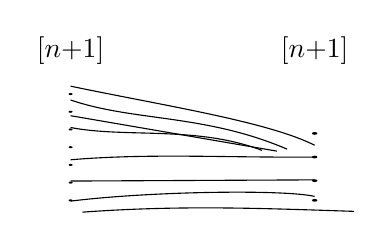
\begin{tikzpicture}[x=1cm,y=0.5cm]
\node at (0,3.8) {$[n\deleted{\unsure{+1}}]$};
\node at (3.1,3.8) {$[\unsure{n}\deleted{\unsure{+1}}]$};
\foreach \y in {0,0.45,0.9,1.35,1.8,2.25,2.7}
{\fill (0,\y) circle (.026);}\foreach \y in {0,.5,1.1,1.7}{\fill (3.1,\y) circle (.035);}
\draw (0,2.9) .. controls (1.2,2.4) and (2.5,2) .. (3.1,1.4);
\draw (0,2.55) .. controls (.8,2) and (1.7,2.2) .. (2.75,1.3);
\draw (0,2.15) -- (2.62,1.25);
\draw (0,1.85) .. controls (.7,1.58) and (1.6,1.9) .. (2.43,1.27);
\draw (0,1.03) .. controls (1,1.2) and (2,1.08) .. (3.1,1.1);
\draw (0,.49) -- (3.1,.52);
\draw (0,-.02) .. controls (1,.23) and (2.7,.28) .. (3.1,.1);
\draw (.15,-.3) .. controls (1.4,-.12) and (2.4,-.2) .. (3.6,-.28);
\end{tikzpicture}}

\uuline{Alexander-Whitney}
\[
\begin{aligned}
\widehat X_{n,n}&\longrightarrow\bigoplus X_{ij}\\
x_{n,n}&\longrightarrow\sum_{i=0}^{n}(-1)^i d_0^{n-i}\widehat{d'^{i}}x_{n,n}
\end{aligned}
\]
\diagram{\begin{tikzcd}[ampersand replacement=\&]
\underbrace{C^i(X,A)}_{f}\otimes\underbrace{C^j(X,B)}_{g}\arrow[r,Rightarrow] \& C^{i+j}(X\times X,A\otimes B)\arrow[dr] \&\\
\mathbb ZX\otimes\mathbb ZX \& \mathbb Z(X\times X)\arrow[l,Rightarrow] \& C^{i+j}(X,A\otimes B)
\end{tikzcd}}
\(\widehat{d}\) signifie le dernier op face

\(d'\) second op simpl.
\[
\widehat{d'^{i}}=d'^{n}d'^{n-1}\ldots d'^{n-i+1}
\]
\(EZ^{-1}\Rightarrow EZ\)

Cup-produit \(\left\{\begin{aligned}
&h(x_1,\ldots,x_{n+1})\\
&=\sum(-1)f(x_1,\ldots,x_i)g(x_{i+1},\ldots,x_n)
\end{aligned}\right.\)

\uline{Associatif}\quad (non-commutatif mais comm à homotopie près) \(\Rightarrow H^*(X,R)\) est anticom.
% archive sheet number: 358
\scanpage{358}
\diagram{\begin{tikzcd}[ampersand replacement=\&]
K(\unsure{\mathbb Z|Z},i)\times K(\mathbb Z,j)\arrow[r]\arrow[d] \& K(\mathbb Z,i+j\\
K(\mathbb Z,i)\otimes K(\mathbb Z,j)\arrow[ur,"f"] \&
\end{tikzcd}}

Il suffit de construire \(Nf\)
\diagram{\begin{tikzcd}[ampersand replacement=\&]
N\bigl(K(\mathbb Z,i)\otimes K(\mathbb Z,j\bigr)\arrow[dr,"E.Z."'] \& \& NK(\mathbb Z\unsure{\,|,}i+j)=\mathbb Z[i+j]\\
\& {\begin{gathered}NK(\mathbb Z,i)\otimes NK(\mathbb Z,j)\\[-2pt]\shortparallel\\[-2pt]\mathbb Z[i]\otimes\mathbb Z[j]\end{gathered}}\arrow[ur] \&
\end{tikzcd}}

\diagram{\begin{tikzcd}[ampersand replacement=\&,execute at end picture={\draw (current bounding box.north west) -- (current bounding box.south east);\draw (current bounding box.south west) -- (current bounding box.north east);}]
{\deleted{\left(\begin{gathered}\mathrm{Inv}^{G}(S\mathfrak g^*)\\ H^*(G,L\mathrm{Sym}\mathfrak g^{\unsure{\vee|*}})\end{gathered}\right.}}\arrow[r,Rightarrow] \&
{\deleted{\left.H^*(BG)\right)}}
\end{tikzcd}}
% Two crossing pencil lines cancel the entire parenthesized diagram, arrow included.
% archive sheet number: 359
\scanpage{359}
\mspage{EZ 2}
Cor
\diagram{\begin{tikzcd}[ampersand replacement=\&]
\Sigma_n\arrow[r] \& E\Sigma_n=\deleted{\unsure{K(\Sigma_n,1)}}\arrow[d,no head]\\
\& K(\Sigma_n,1)
\end{tikzcd}}
\[
W_n=\mathbb ZE\Sigma_n\xrightarrow{\sim}\mathbb Z
\]
\inserted{résol de \(\mathbb Z\) par des \(\Sigma_n\)-modules \deleted{plats} libres.}

Cor du th
\[
W_n\xrightarrow{\unsure{\urcorner|?|\sim}}\mathrm{Hom}^{\unsure{'|\bullet}}(\deleted{\unsure{\mathbb ZX\otimes\mathbb ZX}}\;\mathbb ZX\times X\times\ldots,\ \mathbb ZX\otimes\ldots\otimes\mathbb ZX)
\]
D'où par adjonction une fleche
\[
\begin{aligned}
W_n\otimes\mathbb Z(X\times\ldots\times X)&\xrightarrow{\lambda}\mathbb ZX\otimes\mathbb ZX\ldots\otimes\mathbb ZX\\
(\text{resp. }W_n\otimes\mathbb ZX\otimes\ldots\otimes\mathbb ZX&\longrightarrow\mathbb Z(X\times\ldots\times X)\;)
\end{aligned}
\]
Ceci exprime l'homotopie-commutativité \unsure{enoncée|annoncée} \(+\) haut

\uline{Ex \(n=2\)}\quad 1) exemple topologique :
\[
\begin{aligned}
X\times X&\xrightarrow{m} X\qquad\text{homotopiq com}\\
\Sigma_2\ \text{équiv}\quad I\times X\times X&\longrightarrow X \qquad\ldots\longrightarrow\\
+\ \text{fort}\quad E\Sigma_2\times X^2&\longmapsto X\qquad \Sigma_2\ \text{equiv}
\end{aligned}
\]
classiquemen \(\quad E\Sigma_n\times X^n\longrightarrow X\)\quad relevant la mult itérée

\(\Sigma_2\) agit sur \(S^n\) par action antipodale
\[
\begin{aligned}
&\downarrow\hspace{4em} E\Sigma_2=\varinjlim S^n\\
&\mathbb P^n(\mathbb R)\qquad x,y\qquad\deleted{xy=yx}\\
&&xyx^{-1}y^{-1}
\end{aligned}
\]
\diagram{\begin{tikzcd}[ampersand replacement=\&]
S^1\times X^2\arrow[r]\arrow[d] \& X\\
S^2\times X^2\arrow[ur,"\Sigma_2\text{-equiv}"] \&
\end{tikzcd}}
etc \ldots

\figure{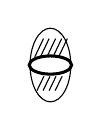
\begin{tikzpicture}[scale=.55]
\draw (0,0) ellipse (.47 and .85);
\draw[line width=1.1pt] (0,0) ellipse (.49 and .21);
\foreach \a in {-0.28,-0.15,0,.14,.27}{\draw (\a-.08,.19) -- (\a+.12,.61);}
\foreach \a in {-.23,-.09,.05,.19}{\draw (\a-.08,-.59) -- (\a+.08,-.26);}
\end{tikzpicture}}

\(\Sigma_n\times\Sigma_n=\Sigma_n\)
\diagram{\begin{tikzcd}[ampersand replacement=\&]
{\deleted{\unsure{E\Sigma_n\times(E\Sigma_j\times X^j)^n|E\Sigma_n\times(E\Sigma_j\times X)^n}}}\arrow[d] \&
{E(\Sigma_n\int\Sigma_j)\times(X_1^0\ldots X_j^0)\times X_1^1\ldots X_j^1\times\ldots X_1^n\times\ldots\times X_{j}^n}\arrow[l]\arrow[dd]\\
X^n \& {}\\
X \& E\Sigma_n\times X^n\arrow[l,"?"']
\end{tikzcd}}
Cor : les enoncés précédents impliquent que lorsque \(X\) est un H esp sat à ce genre de cdn de commutativité à homotopie près, alors les chains \(\mathbb ZX\) ont ce
\[
W_n\otimes\mathbb ZX^{\otimes n}\xrightarrow{\Sigma_n\ \text{equiv}}\mathbb ZX^{\unsure{\epsilon|e|\otimes}}\longrightarrow
\]
t.q induise la mult des chains
\[
\mathbb ZX^{\otimes n}\xrightarrow[\text{shuffles}]{EZ}\mathbb Z(X^n)\xrightarrow{\mathbb Z(m)}\mathbb ZX
\]
Constr des operations de Steenrod :
\[
\mathbb ZX\unsure{\longrightarrow|\rightrightarrows}\qquad A\ \text{un anneau de car}\ p
\]
\[
\deleted{\unsure{f\in}}Z^n(X,A)\qquad(\widetilde{\mathbb ZX})\xrightarrow{f} A[n]
\]
\diagram{\begin{tikzcd}[ampersand replacement=\&,column sep=small]
W_p\otimes\mathbb Z(X^p)\arrow[r,"\lambda"] \& \widetilde{\mathbb ZX}^{\otimes p}\arrow[r,"f^{\otimes p}"] \& A[n]^{\otimes p}\arrow[r,"\mu"] \& A[pn]\\
W_p\otimes\mathbb ZX\arrow[u,"\Delta"]\arrow[urrr,"\Sigma_n\ \text{equiv}"'] \& \& \&
\end{tikzcd}}
\margin{\fbox{\(\substack{\text{cf Steenrod p \uline{39}}\\ \text{\uline{Coh} ops}}\)}}

(avec action triv sur \(\mathbb ZX\))
\(\deleted{\unsure{W_{\Sigma_n}}}\)
\[
\begin{aligned}
Pf&=\mu\circ f^{\times p}\circ\lambda\ \in{}_{\Sigma_n}H^{pn}(\mathbb Z(X^p),A)\\
&\hspace{12em}\downarrow\\
\bigl(W_n\otimes\mathbb ZX/\Sigma_n&=\mathbb ZX\otimes\mathbb ZK(\Sigma_n,1)\qquad{}_{\Sigma_n}H^{\unsure{p\times n|pn}}(X,A)\\
\Sigma_n&\hspace{14em}\shortparallel\\
&\hspace{9em}H^*(K(\Sigma_{p})\deleted{\unsure{\times}}\times X,A)\\
&\hspace{14em}\shortparallel\\
\text{Kunneth}\quad &H^*(\Sigma_p)\otimes_{\mathbb F_p}H^*(X,A)
\end{aligned}
\]
% archive sheet number: 360
\scanpage{360}
\mspage{EZ 3}
Les applications shuffles et A-W sont \uline{assoc}

\(\left(\begin{aligned}
&\text{et \uline{shuffles} est (anti)-commutative}\\
&\text{A-W \quad - \quad est seulement comm à homotopie près.}
\end{aligned}\right.\)

On peut exprimer ceci avec des diagrammes \unsure{d'objets} \unsure{trisimpliciaux}

\margin{Ref Illusie \uline{thèse.}}
\diagram{\begin{tikzcd}[ampersand replacement=\&]
X_{***}\arrow[r,"N_{\unsure{123|12|**}}"]\arrow[d,"\Delta_{12}"'] \& X_{\bullet\bullet\bullet}\arrow[r,"\int_{12}"] \& X_{\bullet\bullet}\arrow[d,"\int"]\\
X_{**}\arrow[r,"N"] \& X_{\bullet\bullet} \& X_\bullet
\end{tikzcd}}

Clair pour \(\underline{\mathbb ZX}\).
\[
\deleted{\unsure{\mathbb ZX\otimes\mathbb ZX\otimes\mathbb ZX\otimes\mathbb ZX}}
\]
L'enoncé de commutativité s'enonce comme suit : \hfill \(X\) ens simpl
\[
\begin{aligned}
&\deleted{\mathrm{Hom}(\mathbb ZX\otimes\mathbb ZX,\mathbb Z(X\times X))}\\
&\mathrm{Hom}^{\unsure{\bullet|'}}\bigl(\widetilde{\mathbb Z(X\times X)},\widetilde{\mathbb ZX}\otimes\widetilde{\mathbb ZX}\bigr)\longrightarrow\mathbb Z
\end{aligned}
\]
\(\Sigma_2\) agit sur ce complexe
\[
\begin{aligned}
&\nearrow\quad\mathrm{Hom}\bigl(\mathbb Z(X_0\times X_0)\xrightarrow{\sim}\mathbb ZX_0\otimes\mathbb ZX_0\bigr)\longrightarrow\mathbb Z\\
&\hspace{4em} X\longrightarrow\mathrm{pt}\ \deleted{\longrightarrow}\\
&\mathrm{Hom}\bigl(\mathbb Z(\ ,\ ),\widetilde{\mathbb Z(\ )}\otimes\widetilde{\mathbb Z(\ )}\bigr)\longrightarrow\mathbb Z
\end{aligned}
\]
\uline{Theorème} (Dold) : \textquotedblleft{} \unsure{Ueber|Über} Steenrodsche operationen \ldots\textquotedblright

Pour tout \(X\), Ce complexe
\[
\left.\begin{aligned}
\mathrm{Hom}^{\unsure{'|\bullet}}\bigl(\mathbb Z(X\ldots\times X),\mathbb Z(X)\otimes\ldots\otimes\mathbb ZX\\
\mathrm{Hom}^{\unsure{'|\bullet}}\bigl(\mathbb ZX\otimes\ldots\otimes\mathbb ZX,\mathbb Z(X\times\ldots\times X)
\end{aligned}\right\}
\]
est une \unsure{resolution|résolution} libre de \(\mathbb Z\) dans la cat des \(\Sigma_n\)-modules

\inserted{pour \(X\) variable}

On tronque pour avoir un complexe de chaines
% archive sheet number: 361
\scanpage{361}
\mspage{EZ \deleted{\unsure{2|3}}\unsure{3|9|4}}
\[
\begin{aligned}
f\in H^n(X,A)&\Rightarrow Pf\in{}_{\Sigma_n}H^{pn}(E\Sigma_n\times X^p,A)
\Rightarrow\Delta Pf\in H^{pn}(K(\Sigma_p,1)\times X,A)\\
&\hspace{19em}\shortparallel\\
&\hspace{11em}H^{\unsure{\lambda|*}}(K(\Sigma_p,1)\otimes_{\mathbb F_p}H^*(X,A)\\
&\hspace{12em}\unsure{\circ}\quad\deleted{\unsure{\{e_\alpha\}}}\\
e_\alpha&\in H_{\alpha}(K(\Sigma_p,1))\hspace{8em}\swarrow\\
&\hspace{7em}D_i x\in H^{pn-i}(X,A)
\end{aligned}
\]
\[
\underline{P^i x}=(-1)^{(\ \ )}D_{\unsure{f(i)|k(i)}}.
\]
Ce reindexage est ce qui donne la formule de Cartan

En fait on considere \(\unsure{\mathbb Z_p|Z_p}\subset\Sigma_p\) et on travaille avec la coh du groupe cyclique
% archive sheet number: 362
